\documentclass[journal,compsoc]{IEEEtran}

\usepackage{amsmath,amssymb,amsfonts}
\usepackage{algorithmic}
\usepackage{graphicx}
\usepackage{textcomp}
\usepackage{xcolor}
\usepackage{booktabs}
\usepackage{url}
\usepackage{hyperref}
\usepackage{cite}
\usepackage{microtype}

\hypersetup{
    colorlinks=true,
    linkcolor=black,
    citecolor=black,
    urlcolor=black
}

\begin{document}

\title{Advanced False Data Injection Attacks and Next-Generation Defenses in Cyber-Physical Power Systems: A Comprehensive Technical Review and Orchestration Framework}

\author{Manas~Jain
\thanks{M. Jain is with the Department of Artificial Intelligence and Data Science, Indian Institute of Information Technology Sri City, Chittoor 517646, India (e-mail: manas.j@iiits.in).}}

\markboth{IEEE Communications Surveys \& Tutorials,~Vol.~XX, No.~XX,~2026}%
{Jain: Advanced FDI Attacks and Next-Generation Defenses in Cyber-Physical Systems}

\maketitle

\begin{abstract}
Modern cyber-physical power systems increasingly depend on pervasive sensing, multi-channel communications, and automated distributed control. While this deep cyber-physical coupling delivers unprecedented operational efficiency, it fundamentally exposes critical infrastructure to sophisticated False Data Injection (FDI) attacks. Over the past decade, attack models have evolved from classical residual-bypass formulations into completely stealthy, data-driven, blind, and adversarially crafted attacks that evade both conventional residue-based Bad Data Detection (BDD) and contemporary machine-learning detectors. In response, defensive paradigms are undergoing an architectural shift toward resilient, adaptive, and explainable multi-tier frameworks. 

This paper presents a comprehensive technical review and methodological synthesis of advanced FDI attacks and next-generation defense mechanisms in cyber-physical systems (CPS). We formulate a unified mathematical threat taxonomy spanning adversary knowledge, physical capabilities, and evasion mechanisms across twelve canonical attack classes. Furthermore, we examine the integration of Generative AI (GAI) for proactive attack synthesis, Centralized Training with Decentralized Execution (CTDE) Multi-Agent Deep Reinforcement Learning (MARL) for autonomous detection and mitigation, and Large Language Model (LLM) orchestration for explainable control-room decision support. Across nine structural and theoretical blueprints, we formalize the plant dynamics, closed-loop resilience, CTDE policy optimization, and hierarchical edge--fog--cloud deployment, establishing an actionable foundation for next-generation CPS security.
\end{abstract}

\begin{IEEEkeywords}
False data injection attack (FDIA), cyber-physical systems (CPS), multi-agent reinforcement learning (MARL), generative AI, large language models (LLM), explainable AI (XAI), state estimation, smart grid resilience.
\end{IEEEkeywords}

\section{Introduction}
\IEEEPARstart{M}{odern} electrical power grids, water distribution networks, and transportation systems represent archetypal cyber-physical systems (CPS) wherein discrete computational algorithms and network communications govern continuous physical dynamics \cite{ref1, ref5}. Among the spectrum of cyber vulnerabilities threatening smart grids, the False Data Injection Attack (FDIA), pioneered by Liu et al. \cite{ref29}, poses an existential risk to power system integrity. By compromising sensor telemetry, remote terminal units (RTUs), or communication channels, an attacker introduces carefully calculated bias into state variables (e.g., bus voltage magnitudes and phase angles) while remaining mathematically undetectable to legacy Bad Data Detection (BDD) routines.

While initial research assumed an adversary with complete knowledge of the power network topology and measurement Jacobian matrix $H$, the threat landscape has aggressively diversified. Adversaries exploit low-rank matrix structures \cite{ref48}, principal component analysis (PCA) \cite{ref56}, and blind subspace identification \cite{ref41} to launch attacks without parameter knowledge. Moreover, adversarial perturbations \cite{ref35, ref75} and tensor-completion techniques \cite{ref59} enable evasion of neural-network-based detectors.

To establish enduring resilience, defensive frameworks must transcend static threshold testing. This paper provides an exhaustive review of this evolving threat-defense arms race, structured around nine dedicated architectural and theoretical blueprints.

\section{Overall Architecture and System Model}

\subsection{Theoretical Formulation of CPS Plant Dynamics}
The CPS is modeled as a coupled discrete--continuous stochastic dynamical system. The physical plant evolves according to:
\begin{equation}
x_{t+1} = f(x_t, u_t, w_t), \qquad y_t = h(x_t) + a_t + v_t,
\label{eq:plant_model}
\end{equation}
where $x_t \in \mathbb{R}^n$ represents the physical state vector, $u_t \in \mathbb{R}^m$ is the control input, $w_t \sim \mathcal{N}(0, Q)$ denotes process disturbance, $y_t \in \mathbb{R}^p$ is the sensor measurement vector, $a_t \in \mathbb{R}^p$ is the malicious FDI attack vector, and $v_t \sim \mathcal{N}(0, R)$ denotes measurement noise.

\begin{figure*}[t]
\centering
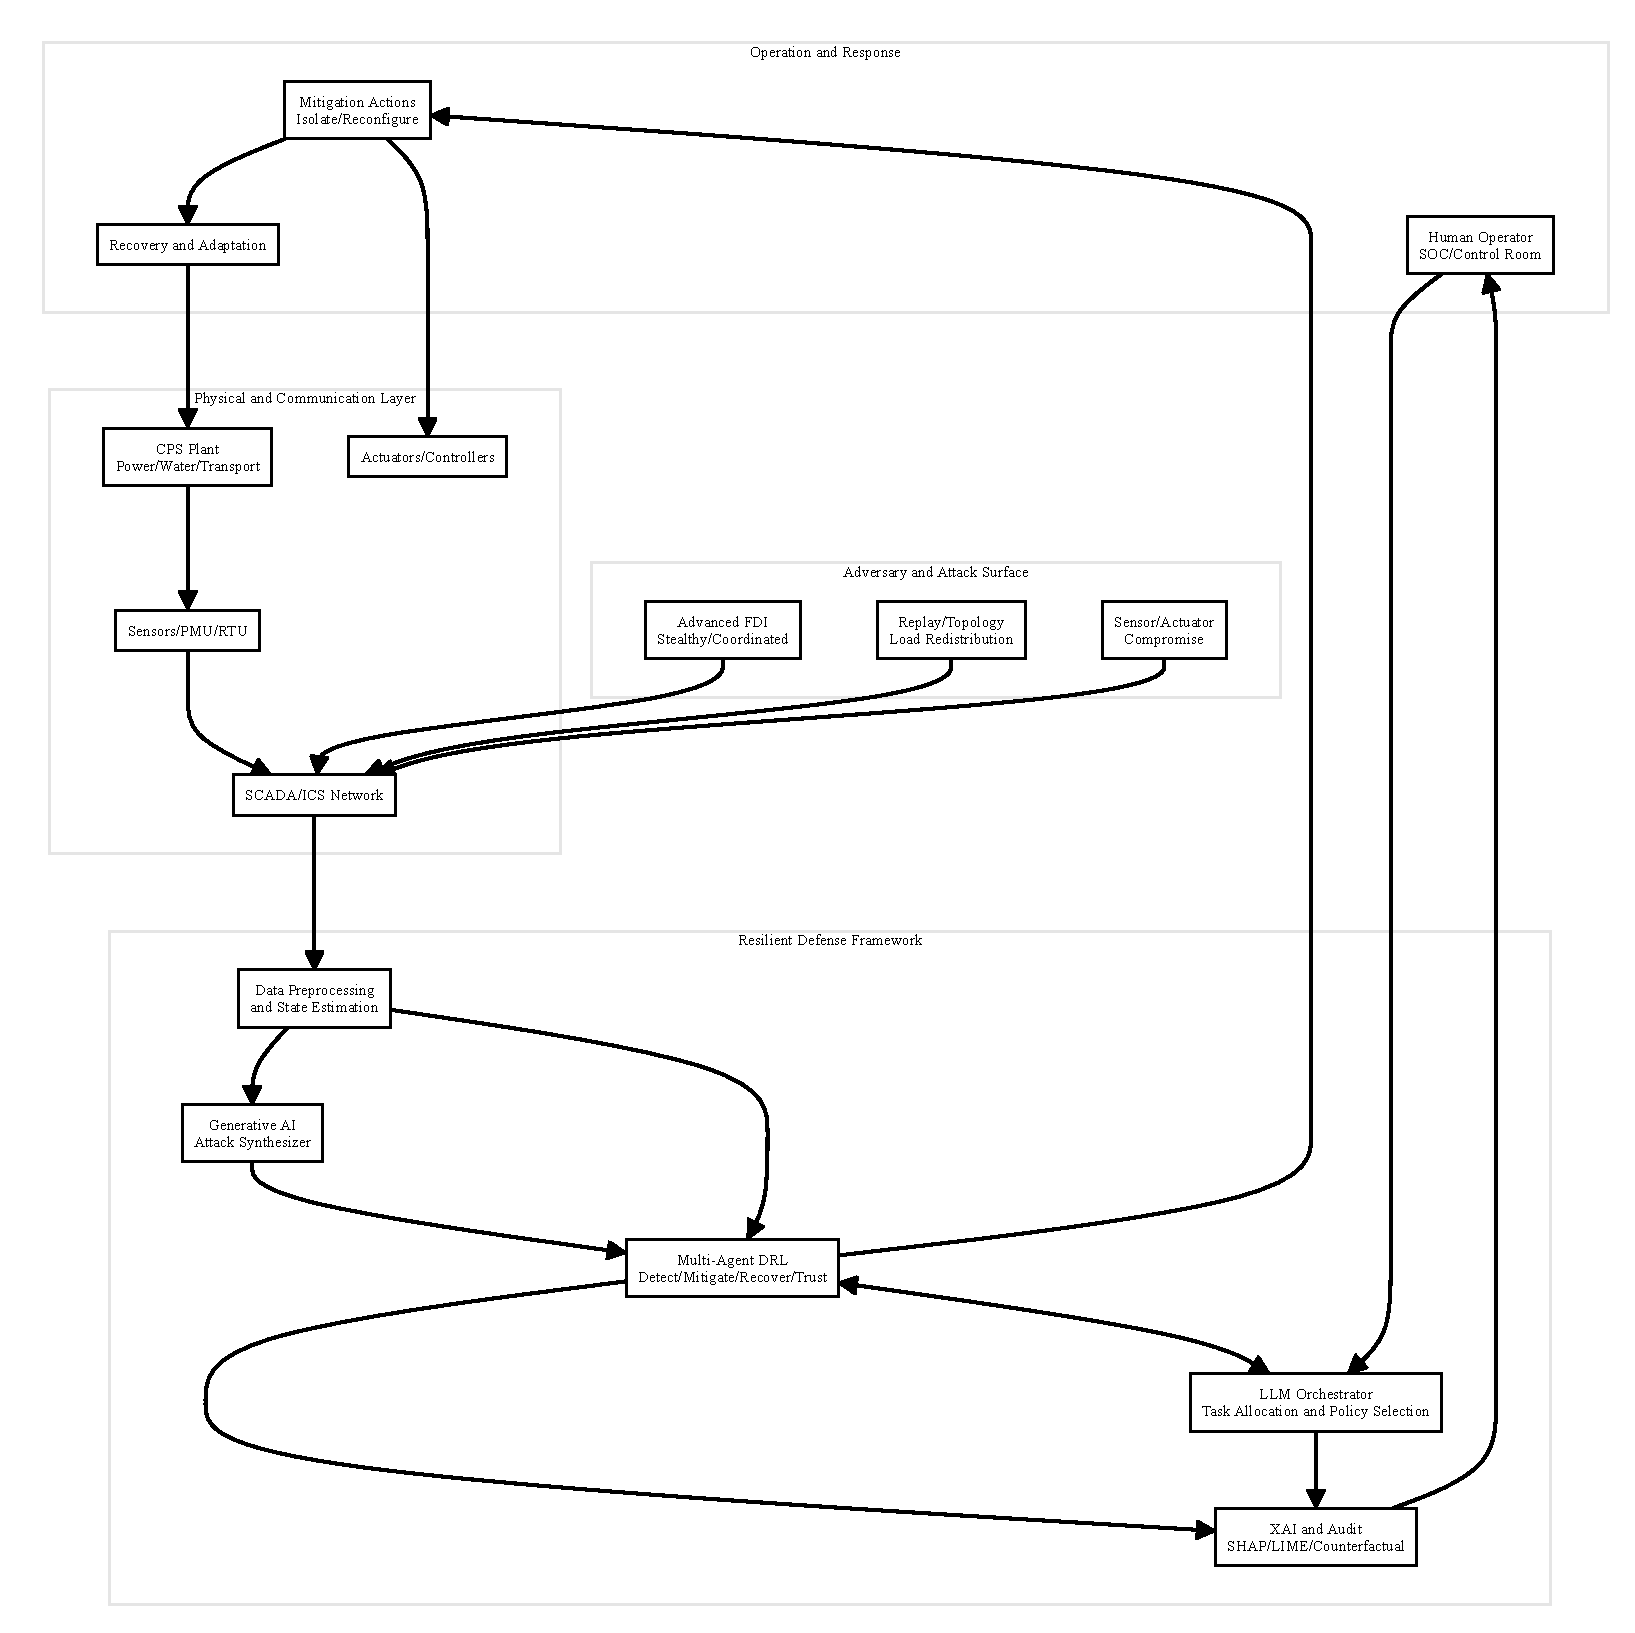
\includegraphics[width=\textwidth]{figures/fig1_overall_architecture.pdf}
\caption{Overall resilient cyber-physical defense architecture across Physical, Adversary, Defense, and Operational layers.}
\label{fig:overall_arch}
\end{figure*}

The defense objective is to preserve system stability, observability, and optimal control under arbitrary adversarial inputs. As illustrated in Fig.~\ref{fig:overall_arch}, the proposed framework implements a closed-loop resilient control sequence:
\begin{equation}
\textbf{sense} \longrightarrow \textbf{detect} \longrightarrow \textbf{mitigate} \longrightarrow \textbf{recover} \longrightarrow \textbf{adapt}.
\end{equation}

Generative AI (GAI) addresses the severe data scarcity of labeled stealthy attacks by approximating the conditional attack distribution $p(a_t \mid \text{context})$. Multi-agent deep reinforcement learning (MARL) formulates defense as a partially observable stochastic game (POSG) among cooperative agents. The LLM orchestrator provides hierarchical meta-control, dynamically allocating tasks and selecting response policies. Explainable AI (XAI) ensures human trust and operator accountability in the control room. The layered separation—physical/communication, adversary, defense, and operation—enables modular verification, preventing single-point catastrophic failure.

\section{Threat Model and FDI Attack Taxonomy}

\subsection{Evasion Mechanics in Power System State Estimation}
In linearized power grid state estimation, measurements $z \in \mathbb{R}^m$ relate to voltage angles $x \in \mathbb{R}^n$ via:
\begin{equation}
z = Hx + a + e,
\end{equation}
where $H \in \mathbb{R}^{m \times n}$ is the measurement Jacobian and $e \sim \mathcal{N}(0, \Sigma)$ is Gaussian noise. Standard bad data detection computes the residual $r = \|z - H\hat{x}\|_2$, where $\hat{x} = (H^T \Sigma^{-1} H)^{-1} H^T \Sigma^{-1} z$. A stealthy attack vector $a$ satisfies:
\begin{equation}
a = Hc,
\end{equation}
for an arbitrary non-zero injection vector $c \in \mathbb{R}^n$. Consequently, the corrupted residual equals the uncorrupted residual:
\begin{equation}
r_a = \|z + a - H(\hat{x} + c)\|_2 = \|z - H\hat{x}\|_2 = r,
\end{equation}
completely bypassing conventional $\chi^2$ and Largest Normalized Residual (LNR) detectors \cite{ref29}.

\begin{figure}[t]
\centering
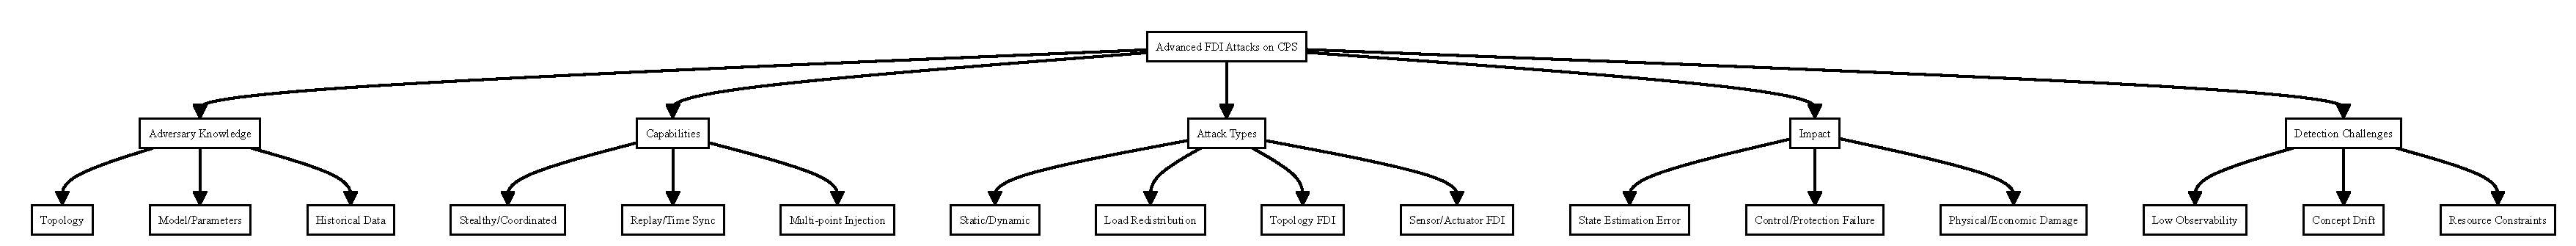
\includegraphics[width=\columnwidth]{figures/fig2_threat_taxonomy.pdf}
\caption{Taxonomy of advanced FDI attacks categorized by knowledge, capabilities, attack modalities, physical impact, and detection bottlenecks.}
\label{fig:threat_taxonomy}
\end{figure}

Fig.~\ref{fig:threat_taxonomy} systematically classifies advanced FDI attacks across five core dimensions:
\begin{enumerate}
    \item \textbf{Adversary Knowledge:} Full topology, line parameter models, or historical telemetry.
    \item \textbf{Adversarial Capabilities:} Complete stealthiness \cite{ref19}, replay synchronization, and multi-point sparse injection \cite{ref44}.
    \item \textbf{Attack Types:} Static/dynamic FDI, load redistribution (LR-FDI), topology manipulation, and actuator tampering.
    \item \textbf{Impact:} State estimation error, economic dispatch distortion, physical equipment tripping, and cascading blackouts.
    \item \textbf{Detection Bottlenecks:} Observability gaps, concept drift under renewable penetration, and millisecond edge computation constraints.
\end{enumerate}

\section{Generative AI Augmentation and MARL Defense}

\subsection{Minimax Adversarial Curriculum Learning}
To counter zero-day attacks, Generative Adversarial Networks (GANs), Variational Autoencoders (VAEs), and diffusion models synthesize worst-case FDI scenarios. The GAN generator $G$ and discriminator $D$ play a zero-sum game:
\begin{equation}
\min_G \max_D \mathbb{E}_{x \sim p_{\text{data}}}[\log D(x)] + \mathbb{E}_{z \sim p_z}[\log(1 - D(G(z)))].
\end{equation}

\begin{figure*}[t]
\centering
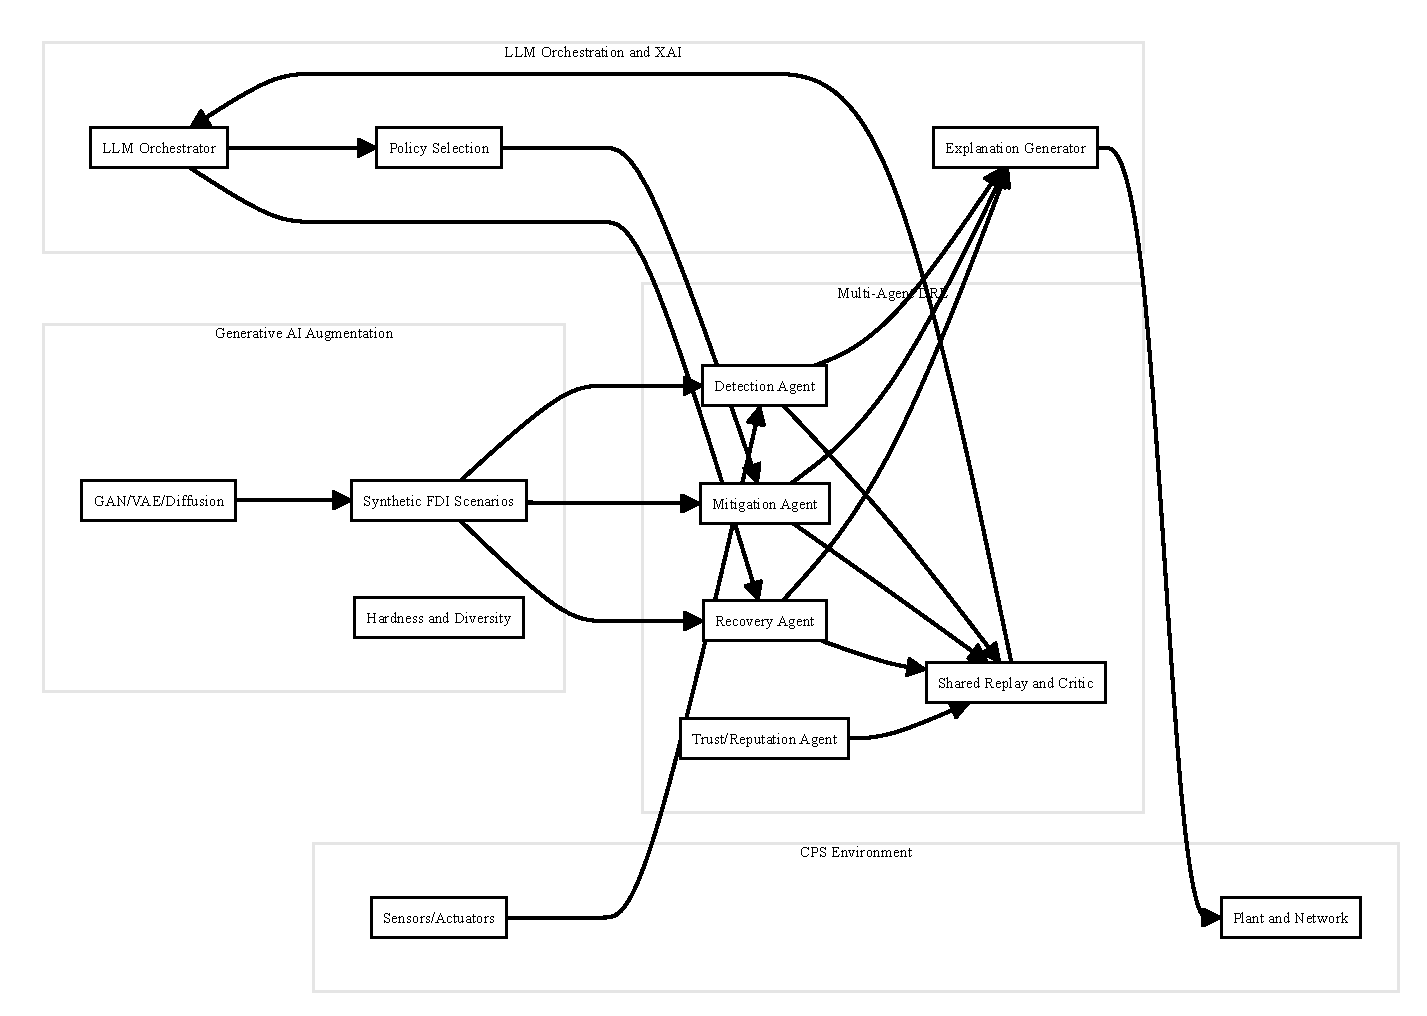
\includegraphics[width=\textwidth]{figures/fig3_gai_marl_framework.pdf}
\caption{Generative AI-augmented Multi-Agent Deep Reinforcement Learning framework with shared replay, centralized critic, and LLM orchestration.}
\label{fig:gai_marl}
\end{figure*}

As shown in Fig.~\ref{fig:gai_marl}, the synthetic attack traces generated by GAI augment the training distribution of four specialized MARL defense agents: Detection, Mitigation, Recovery, and Trust/Reputation. The MARL agents formulate defense as a minimax game:
\begin{equation}
\min_{\pi} \max_{G} \mathbb{E}\left[\sum_{t=0}^{\infty} \gamma^t r_t\right],
\end{equation}
where the reward function $r_t$ penalizes detection latency, false alarms, and control deviation while rewarding rapid physical stabilization.

\section{LLM Orchestration and Explainability Sequence}

\subsection{Hierarchical Meta-Control}
Because power grids operate across disparate timescales—fast protective relays at $10\text{--}50\text{ ms}$ versus secondary AGC and economic dispatch at $2\text{--}10\text{ s}$—the LLM operates exclusively as a slow-timescale meta-controller:
\begin{equation}
\pi_{\text{LLM}}: \mathcal{S} \times \mathcal{C} \longrightarrow \mathcal{A}_{\text{meta}},
\end{equation}
where $\mathcal{S}$ is the aggregated system state summary, $\mathcal{C}$ is context telemetry, and $\mathcal{A}_{\text{meta}}$ selects the low-level policy options executed by local MARL agents.

\begin{figure*}[t]
\centering
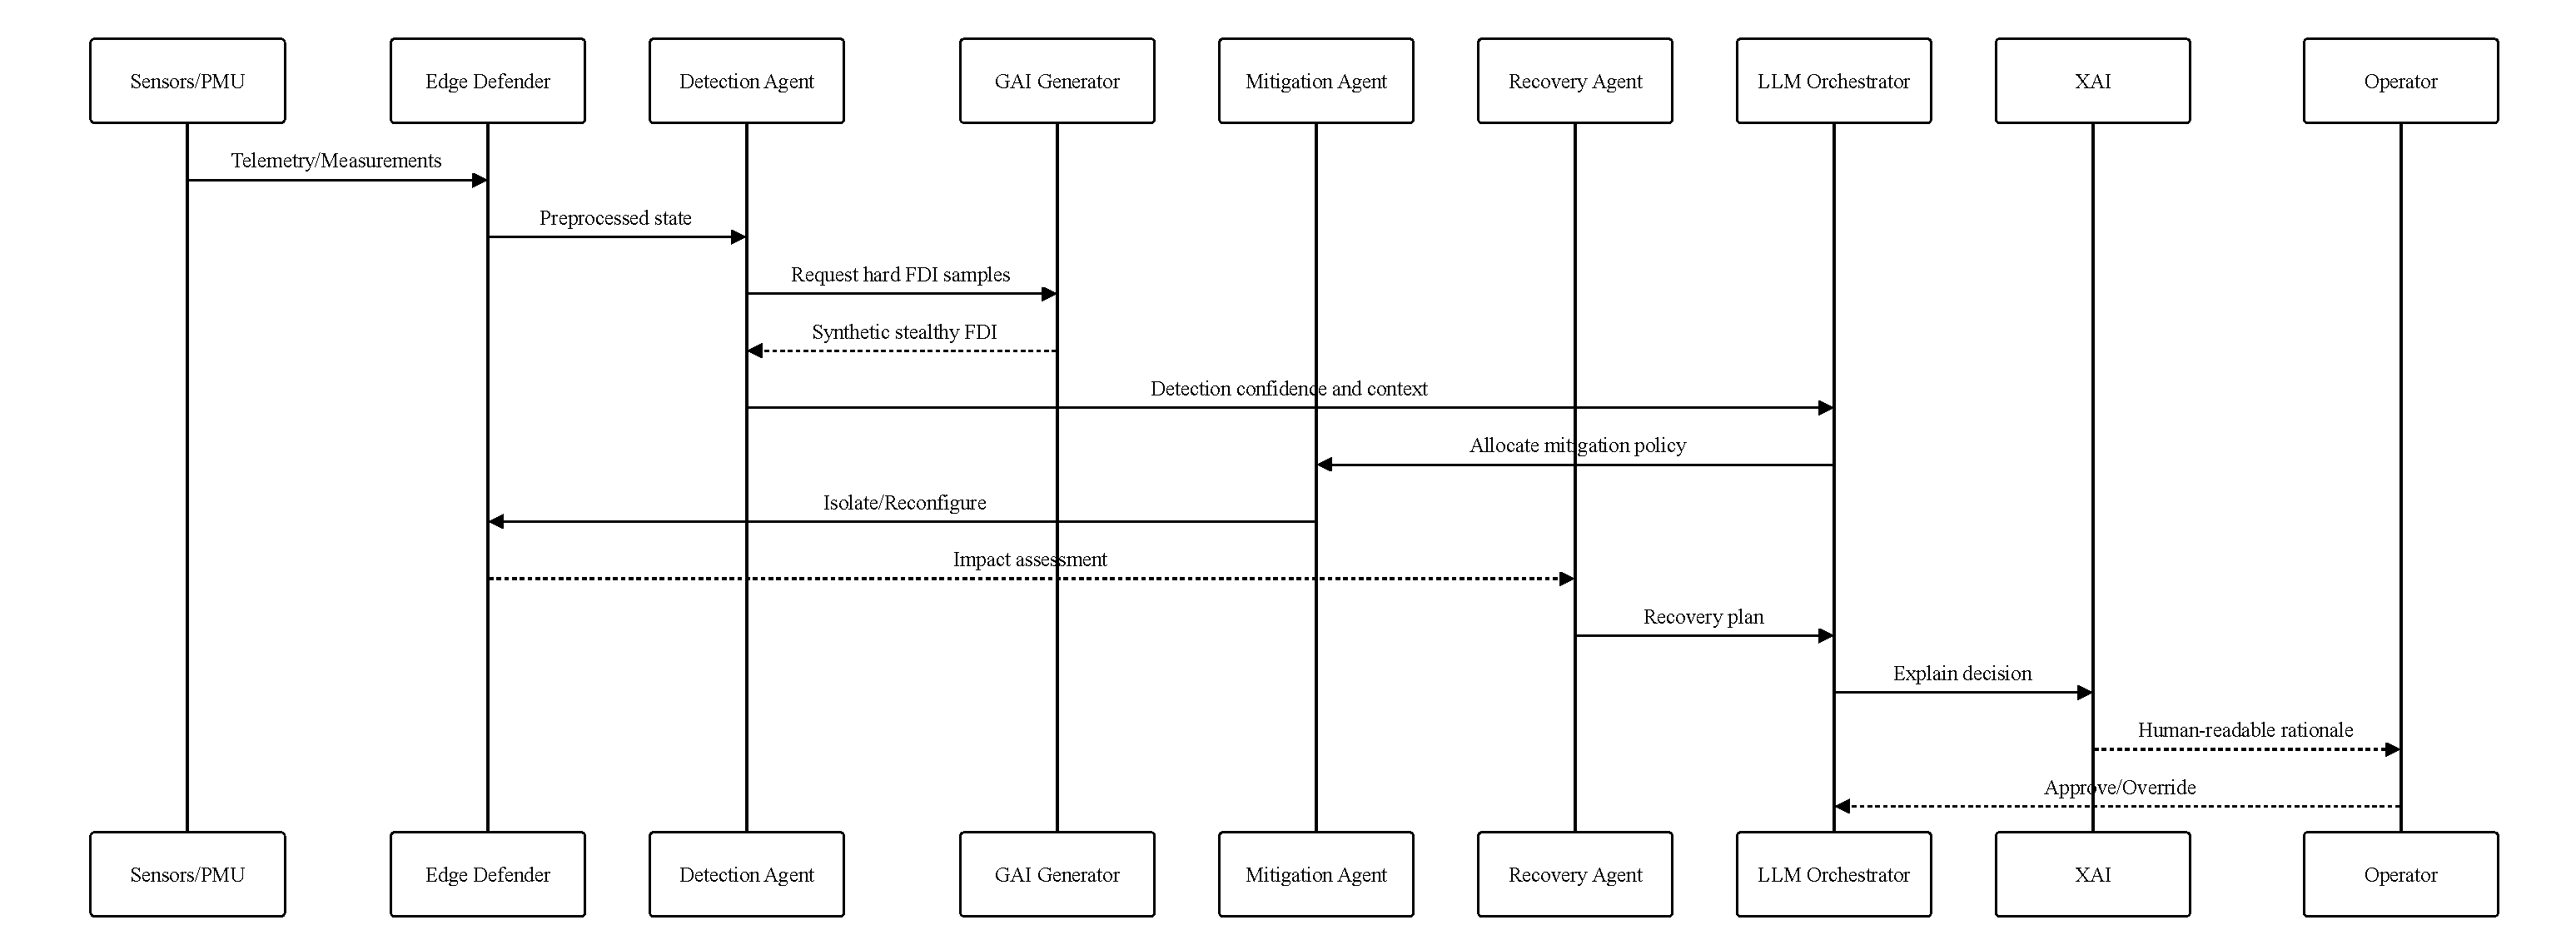
\includegraphics[width=\textwidth]{figures/fig4_llm_orchestration_sequence.pdf}
\caption{Sequence diagram illustrating the closed-loop interaction from PMU sensing to GAI sample generation, MARL action, and LLM-XAI operator approval.}
\label{fig:llm_seq}
\end{figure*}

The full operational sequence is detailed in Fig.~\ref{fig:llm_seq}. Telemetry preprocessed at the edge is verified against GAI attack profiles. Detection confidence triggers LLM mitigation allocation. Mitigation actions isolate affected lines, followed by impact assessment, automated recovery planning, and natural-language explanation generation for control-room operators.

\section{Multi-Agent Interaction Under CTDE}

\begin{figure}[t]
\centering
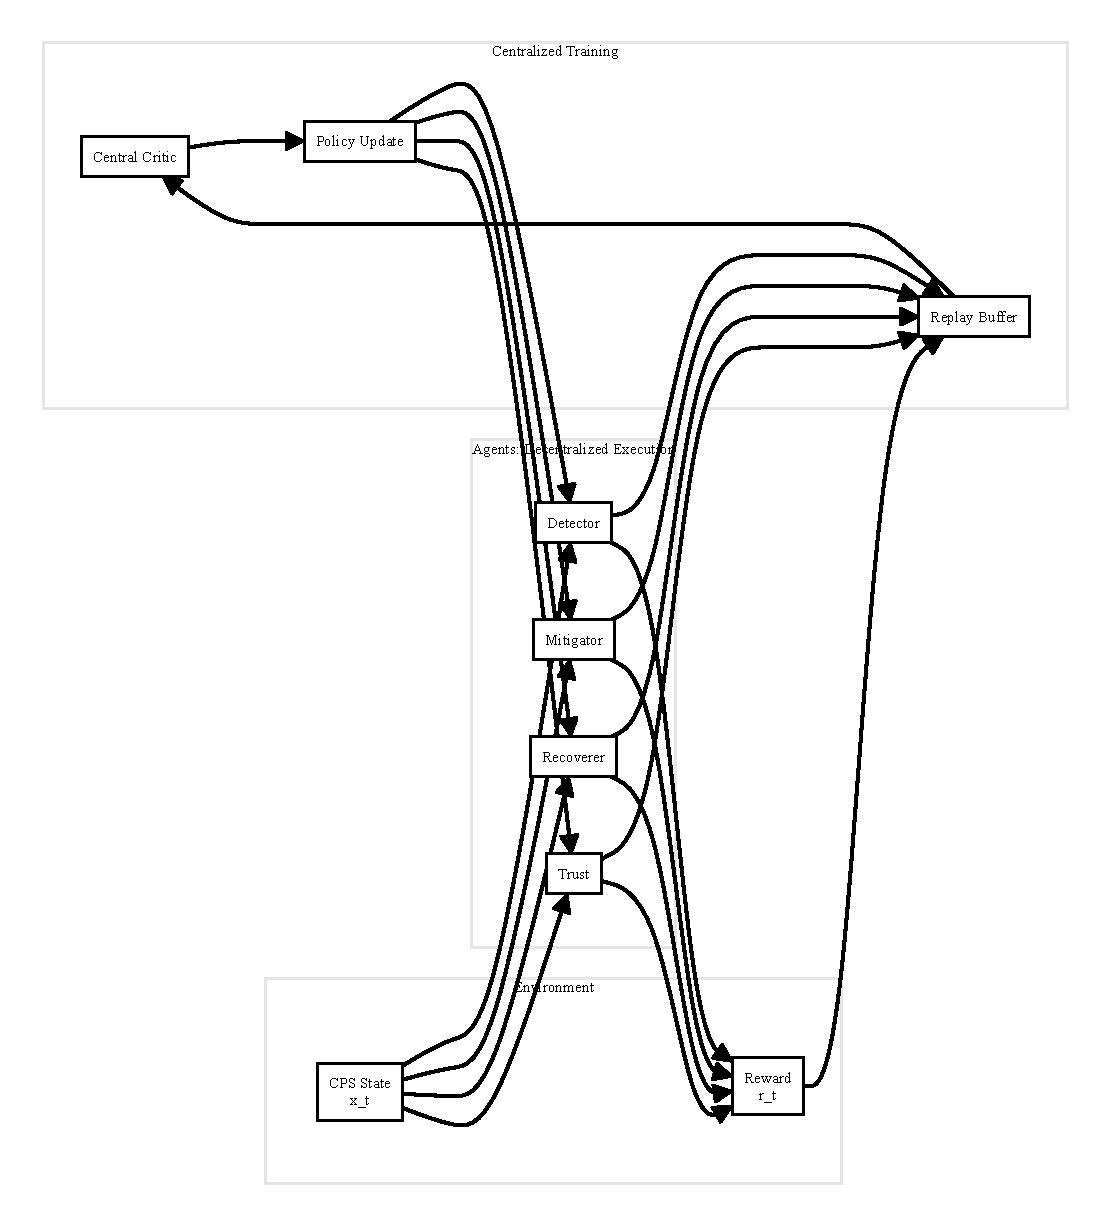
\includegraphics[width=\columnwidth]{figures/fig5_ctde_multi_agent.pdf}
\caption{Centralized Training with Decentralized Execution (CTDE) architecture with centralized critic and local actor policies.}
\label{fig:ctde}
\end{figure}

Multi-agent coordination is governed by Centralized Training with Decentralized Execution (CTDE), addressing non-stationarity and multi-agent credit assignment. As illustrated in Fig.~\ref{fig:ctde}, each agent $i$ observes local telemetry $o_i$ and executes decentralized policy $\pi_i(a_i \mid o_i)$. During offline training, a centralized critic $Q(s, a_1, \dots, a_N)$ conditions on global system state $s$. The policy gradient update for parameter $\theta_i$ is:
\begin{equation}
\nabla_{\theta_i} J = \mathbb{E}\left[\nabla_{\theta_i} \log \pi_i(a_i \mid o_i) Q(s, a_1, \dots, a_N)\right].
\end{equation}
A shared replay buffer stores joint experience tuples, enabling scalable deployment without requiring inter-area high-bandwidth communication during live execution.

\section{End-to-End Pipeline and Explainability Framework}

\begin{figure*}[t]
\centering
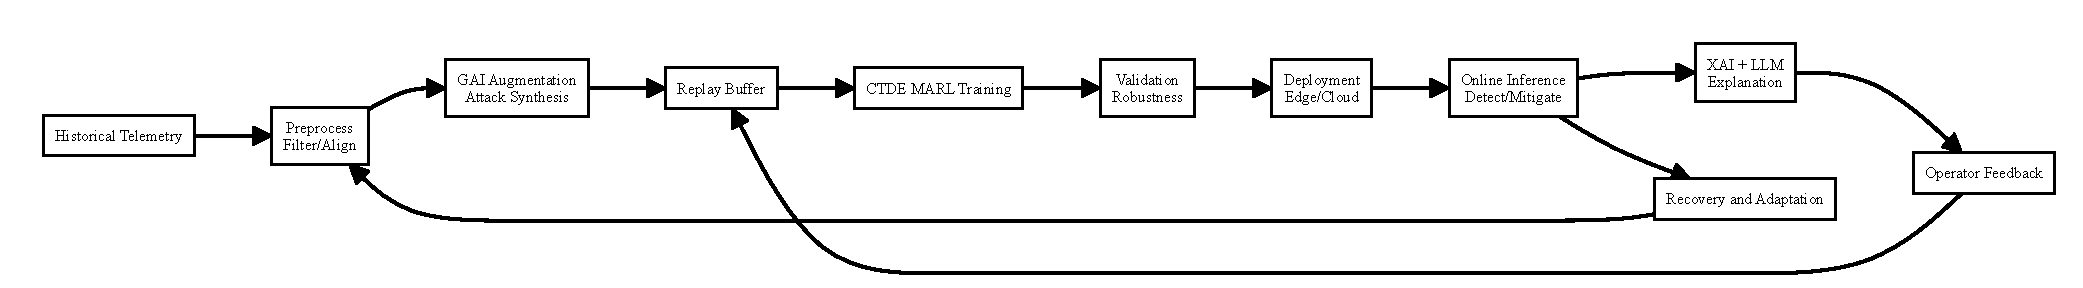
\includegraphics[width=\textwidth]{figures/fig6_training_inference_pipeline.pdf}
\caption{End-to-end training and online inference pipeline integrating data preprocessing, GAI augmentation, CTDE training, deployment, and operator feedback.}
\label{fig:pipeline}
\end{figure*}

\subsection{Continual Training and Online Inference Pipeline}
Fig.~\ref{fig:pipeline} outlines the holistic lifecycle: historical telemetry undergoes alignment and noise filtering before GAI augmentation generates synthetic attack scenarios. Following CTDE training and validation, models deploy across edge gateways and regional substations. Online inference executes millisecond detection and active mitigation, while operator feedback dynamically updates the replay buffer.

\begin{figure*}[t]
\centering
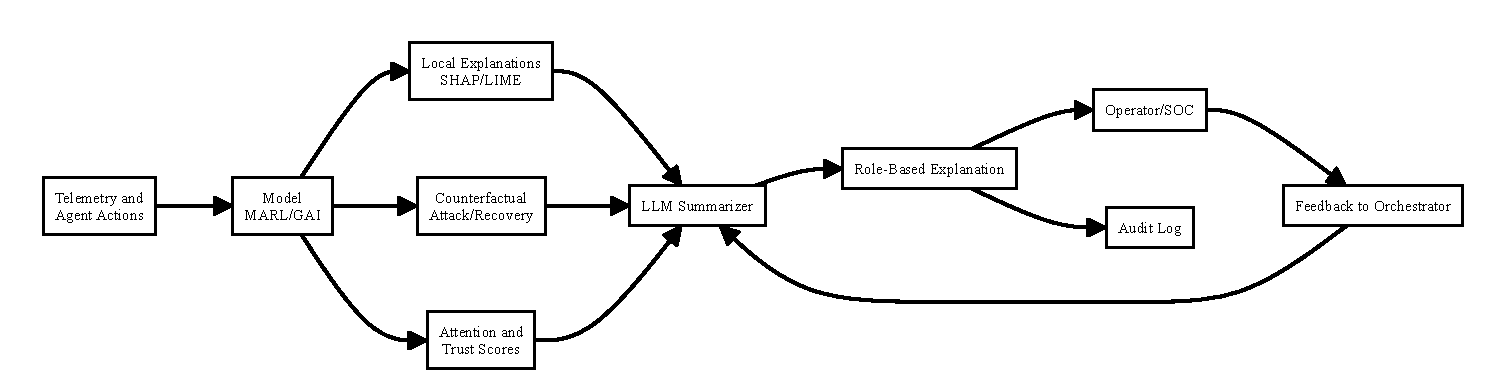
\includegraphics[width=\textwidth]{figures/fig7_explainability_pipeline.pdf}
\caption{Multi-modal explainability pipeline combining SHAP/LIME feature attributions, counterfactual reasoning, and LLM narrative generation.}
\label{fig:xai}
\end{figure}

\subsection{Explainable Decision Support}
Black-box AI models cannot be deployed in safety-critical power grids without interpretability. The explainability pipeline in Fig.~\ref{fig:xai} extracts local feature importances using Shapley values:
\begin{equation}
\phi_i = \sum_{S \subseteq N \setminus \{i\}} \frac{|S|!(|N| - |S| - 1)!}{|N|!} \left[ f(S \cup \{i\}) - f(S) \right],
\end{equation}
alongside counterfactual minimal perturbations $\delta$ such that $f(x + \delta) \neq f(x)$. An LLM summarizer translates these numerical tensors into role-based natural-language operational briefs for control room engineers and compliance auditors.

\section{Deployment Architecture and Finite State Control}

\begin{figure*}[t]
\centering
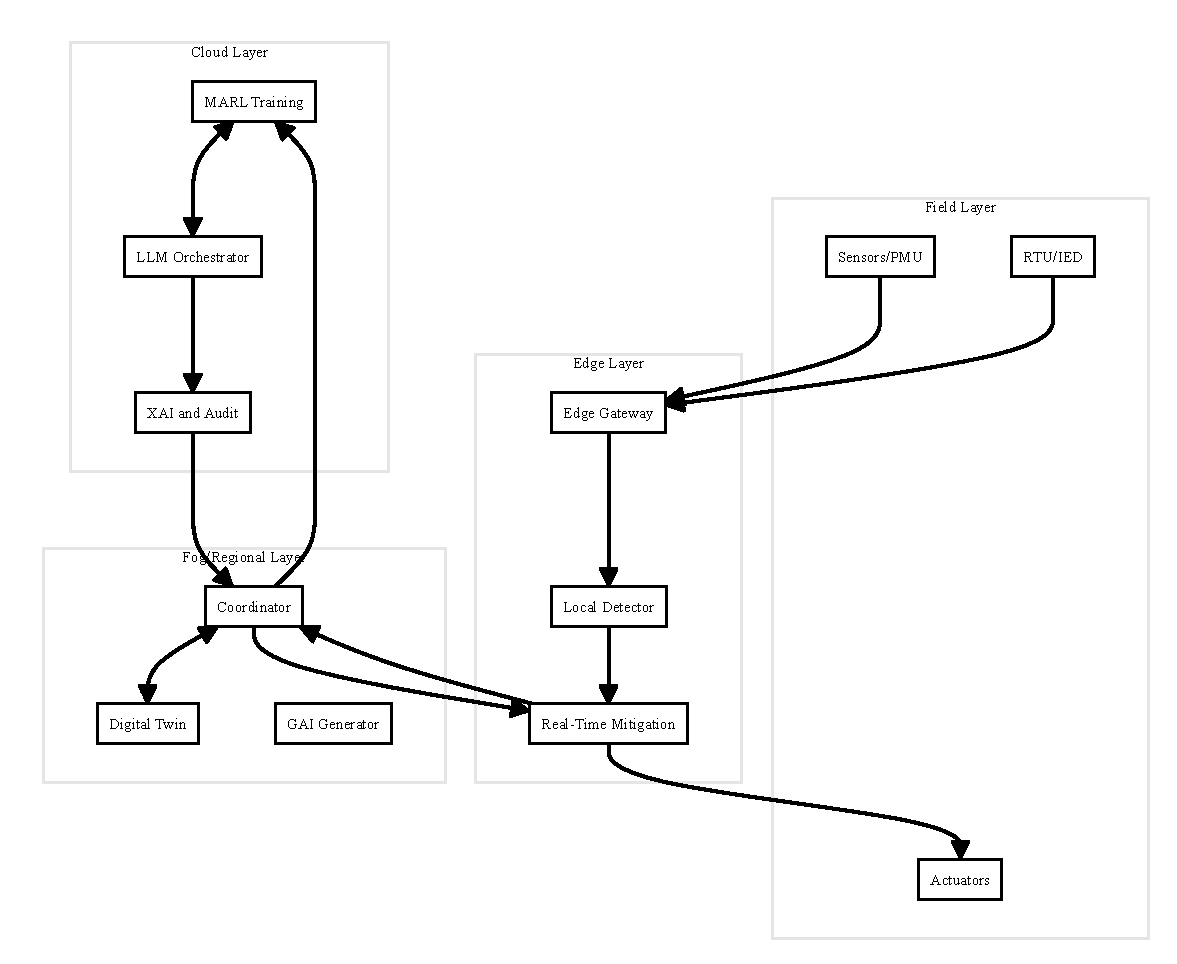
\includegraphics[width=\textwidth]{figures/fig8_edge_fog_cloud_deployment.pdf}
\caption{Three-tier Edge--Fog--Cloud deployment topology across substation field devices, regional control centers, and enterprise cloud.}
\label{fig:deployment}
\end{figure*}

\subsection{Edge--Fog--Cloud Paradigm}
As mapped in Fig.~\ref{fig:deployment}, the system distributes computational workload across three tiers:
\begin{itemize}
    \item \textbf{Edge Layer ($<50\text{ ms}$):} PMU/RTU gateways hosting lightweight neural detectors and automated breaker trip logic.
    \item \textbf{Fog Layer ($100\text{--}500\text{ ms}$):} Regional control centers running digital twin synchronization and local GAI attack generation.
    \item \textbf{Cloud Layer ($>1\text{ s}$):} Centralized utility servers executing heavy CTDE MARL training, LLM orchestration, and long-term audit archiving.
\end{itemize}
Total latency satisfies $T_{\text{total}} = T_{\text{edge}} + T_{\text{fog}} + T_{\text{cloud}}$, with the strict real-time constraint $T_{\text{edge}} \le \tau_{\text{relay}}$.

\begin{figure}[t]
\centering
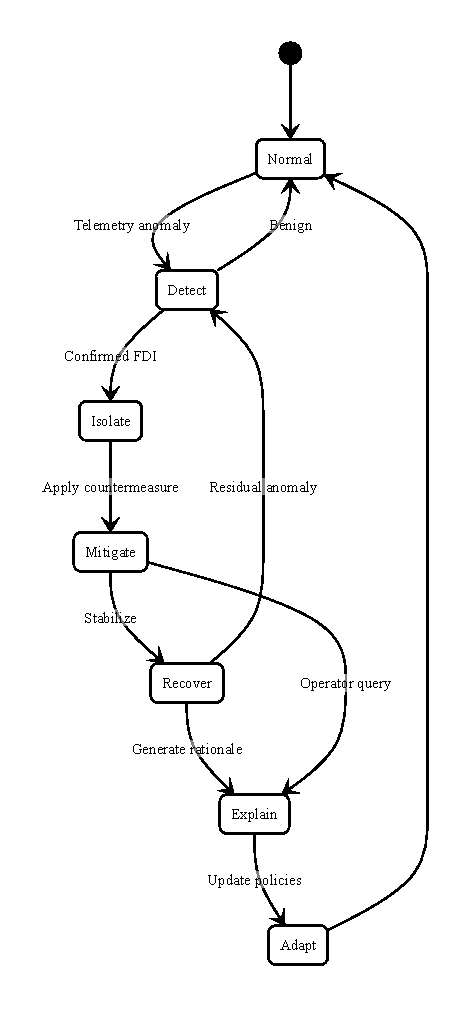
\includegraphics[width=\columnwidth]{figures/fig10_defense_state_machine.pdf}
\caption{Finite state machine governing resilient defense state transitions from Normal to Detect, Isolate, Mitigate, Recover, Explain, and Adapt.}
\label{fig:fsm}
\end{figure}

\subsection{Defense State Machine}
The resilient defense lifecycle is governed by the Finite State Machine (FSM) in Fig.~\ref{fig:fsm}:
\begin{equation}
\mathcal{M} = (\mathcal{S}, \mathcal{A}, \mathcal{T}, s_0, \mathcal{F}),
\end{equation}
with states $\mathcal{S} = \{\text{Normal}, \text{Detect}, \text{Isolate}, \text{Mitigate}, \text{Recover}, \text{Explain}, \text{Adapt}\}$. Transitions are guarded by anomaly thresholds, confirmed FDI classifications, and physical stabilization indicators, guaranteeing bounded recovery time under arbitrary adversarial attack sequences.

\section{Conclusion and Future Directions}
This paper presented a comprehensive survey and architectural framework for securing cyber-physical power systems against advanced False Data Injection attacks. By unifying Generative AI attack synthesis, Multi-Agent DRL with CTDE, and LLM-guided explainable orchestration across an Edge--Fog--Cloud topology, the proposed paradigm bridges the gap between theoretical stealth attacks and practical, resilient grid defense. Future research must address non-linear AC power flow constraints in generative models, quantum-resilient communications, and formal verification of LLM-generated control recommendations.

\bibliographystyle{IEEEtran}
\bibliography{references}

\end{document}
